\documentclass[12pt]{article}
\usepackage{graphicx}
\usepackage{hyperref}
\graphicspath{ {Images/}  }
\begin{document}
	

	\begin{figure}
		
\includegraphics[width=\linewidth]{logo.jpg}	
	\end{figure}

	\title 	{
				COS301\\
				Mini Project\\
				Module Design
		}
	\author {
				Claassen Charles u15216498]\\
                Daubinet Jordan u15260870\\
                Kanda Madimba u17289077\\
                Ngobale Nathan u15110045\\
                Olwage Dedré u15015239\\
                Sargeant Lucian u15225560\\
                Tshela Bongani u14134790\
		}
	\maketitle
	\begin{center}
			\url{https://github.com/ProBlack95/SE-Go-Team}	
	\end{center}
	\newpage
	\tableofcontents
	
	\newpage
		
	\section{Data Module}
	The Data module handles the interactions with the users and the server. Users from different platforms connect to the Access Channel which interacts which interacts with the upstream Manager. The up-stream Manager is the gateway for user requests and responses from the down-stream Manager. The down-stream manager gives all up-stream requests to the server and sends all server responses to the up-stream Manager. The Design patterns which are integrated into the Data Module are: Singleton, chain of responsibility, template, iterator and interface. the Singleton design pattern ensures only one UpStreamManager, DownStreamManager and AccessChannel exist at any time. The chain of responsibility design pattern is used to pass requests up from the user platforms to the server and to pass stream objects from the server to the user platforms. The template design pattern is used to implement different handling methods for the requests of the different concrete plate forms used to connect to the access channel. The iterator design pattern is used for the server to iterate through users when concurrently sending multiple stream objects to different users. The interface design pattern is used to implement how the server acts as an interface for all subsystems.
	
	\subsection{Class Diagram}
        \includegraphics[width=\linewidth]{DataModuleClassDiagram.png}
        \begin{figure}[h]
            \caption{Data Module Class Diagram.}
        \end{figure}
    
    \subsection{Deployment Diagram}
        \includegraphics[width=\linewidth]{DataModuleDeploymentDiagram.png}
        \begin{figure}[h]
            \caption{Data Module Deployment Diagram.}
        \end{figure}
        
    \subsection{Activity Diagram}
        \includegraphics[width=\linewidth]{DataModuleActivityDiagram.png}
        \begin{figure}[h]
            \caption{Data Module Activity Diagram.}
	    This figure describes the methods that the data module might have. The users (iOS/Android/Web) will interact with the system using CRUD (Create Read Update Delete) functionality. The users will send requests(such as adding a user etc.) to the system (upstream) and wait for responses from the system. The system will send responses to the user (downstream) and wait for requests from the user.
        \end{figure}
	
	\subsection{State Diagram}
       \includegraphics[width=\linewidth]{DataModuleStateDiagram.png}
        \begin{figure}[h]
        	\caption{Data Module State Diagram.}
        \end{figure}
	
	\subsection{Use Case Diagram}
        	\includegraphics[width=\linewidth]{DataModuleUseCaseDiagram.png}
        	\begin{figure}[h]
        		\caption{Data Module Use Case Diagram.}
        	\end{figure}
	
	%%%%%%%%%%%%%%%%%%%%%%%%%%%%%%%%%%%%%%%%%%%%%%%%%%%%%%%%%%%%%%%%%%%%%%%%%%
	\section{User Management Module}
	
	\subsection{Class Diagram}
        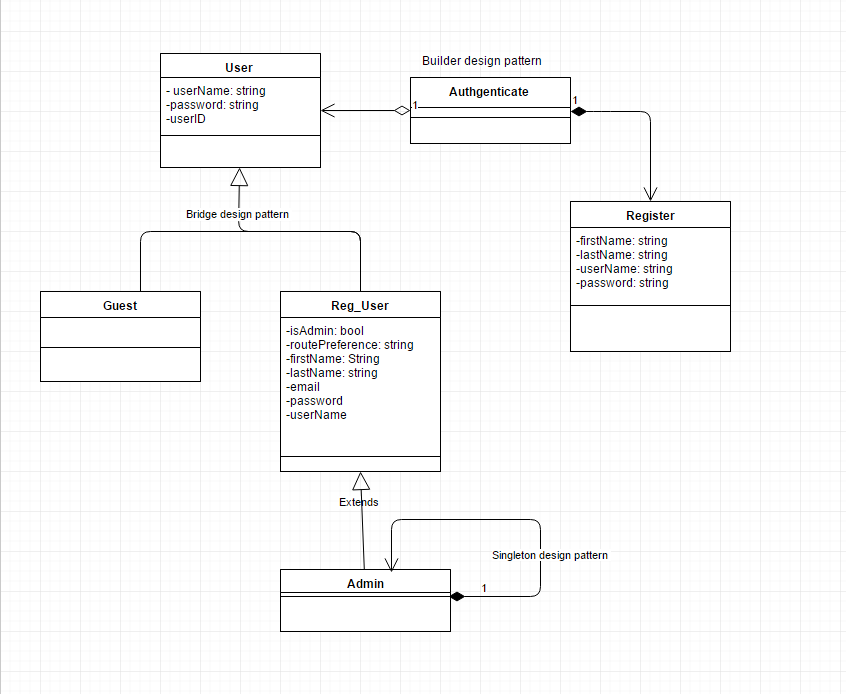
\includegraphics[width=\linewidth]{UserModuleClassDiagram.png}
        \begin{figure}[h]
            \caption{User Management Module Class Diagram.}
        \end{figure}
    
    \subsection{Deployment Diagram}
        \includegraphics[width=\linewidth]{UserModuleDeploymentDiagram.png}
        \begin{figure}[h]
            \caption{User Management Module Deployment Diagram.}
        \end{figure}
        
    \subsection{Activity Diagram}
        \includegraphics[width=\linewidth]{UserModuleActivityDiagram.png}
        \begin{figure}[h]
            \caption{User Management Module Activity Diagram.}
        \end{figure}

    \subsection{Sequence Diagram}
        \includegraphics[width=\linewidth]{UserModuleSequenceDiagram.png}
        \begin{figure}[h]
            \caption{User Management Module Sequence Diagram.}
        \end{figure}

	
	\subsection{State Diagram}
       \includegraphics[width=\linewidth]{UserModuleStateDiagram.png}
        \begin{figure}[h]
        	\caption{User Management Module State Diagram.}
        \end{figure}
	
	\subsection{Use Case Diagram}
        	\includegraphics[width=\linewidth]{UserModuleUseCaseDiagram.png}
        	\begin{figure}[h]
        		\caption{User Management Module Use Case Diagram.}
        	\end{figure}
        	
   %%%%%%%%%%%%%%%%%%%%%%%%%%%%%%%%%%%%%%%%%%%%%%%%%%%%%%%%%%%%%%%%%%%%%%%%%%
   
   \section{Points Of Interest Module}
	
	\subsection{Class Diagram}
        \includegraphics[width=\linewidth]{PointsOfInterestModuleClassDiagram.png}
        \begin{figure}[h]
            \caption{Points Of Interest Module Class Diagram.}
        \end{figure}
    
    \subsection{Deployment Diagram}
        \includegraphics[width=\linewidth]{PointsOfInterestModuleDeploymentDiagram.png}
        \begin{figure}[h]
            \caption{Points Of Interest Module Deployment Diagram.}
        \end{figure}
        
    \subsection{Activity Diagram}
        \includegraphics[width=\linewidth]{PointsOfInterestModuleActivityDiagram.png}
        \begin{figure}[h]
            \caption{Points Of Interest Module Activity Diagram.}
        \end{figure}

    \subsection{Sequence Diagram}
        \includegraphics[width=\linewidth]{PointsOfInterestModuleSequenceDiagram.png}
        \begin{figure}[h]
            \caption{Points Of Interest Module Sequence Diagram.}
        \end{figure}

	
	\subsection{State Diagram}
       \includegraphics[width=\linewidth]{PointsOfInterestModuleStateDiagram.png}
        \begin{figure}[h]
        	\caption{Points Of Interest Module State Diagram.}
        \end{figure}
	
	\subsection{Use Case Diagram}
        	\includegraphics[width=\linewidth]{PointsOfInterestModuleUseCaseDiagram.png}
        	\begin{figure}[h]
        		\caption{Points Of Interest Module Use Case Diagram.}
        	\end{figure}
        	
   %%%%%%%%%%%%%%%%%%%%%%%%%%%%%%%%%%%%%%%%%%%%%%%%%%%%%%%%%%%%%%%%%%%%%%%%%%
   
   \section{Events Module}
	
	\subsection{Class Diagram}
        \includegraphics[width=\linewidth]{EventsModuleClassDiagram.png}
        \begin{figure}[h]
            \caption{Events Module Class Diagram.}
        \end{figure}
    
    \subsection{Deployment Diagram}
        \includegraphics[width=\linewidth]{EventsModuleDeploymentDiagram.png}
        \begin{figure}[h]
            \caption{Events Module Deployment Diagram.}
        \end{figure}
        
    \subsection{Activity Diagram}
        \includegraphics[width=\linewidth]{EventsModuleActivityDiagram.png}
        \begin{figure}
            \caption{Events Module Activity Diagram.}
        \end{figure}

    \subsection{Sequence Diagram}
        \includegraphics[width=\linewidth]{EventsModuleSequenceDiagram.png}
        \begin{figure}[h]
            \caption{Events Module Sequence Diagram.}
        \end{figure}

	
	\subsection{State Diagram}
       \includegraphics[width=\linewidth]{EventsModuleStateDiagram.png}
        \begin{figure}[h]
        	\caption{Events Module State Diagram.}
        \end{figure}
	
	\subsection{Use Case Diagram}
        	\includegraphics[width=\linewidth]{EventsModuleUseCaseDiagram.png}
        	\begin{figure}[h]
        		\caption{Events Module Use Case Diagram.}
        	\end{figure}
   
\end{document}
